\documentclass{article}
\usepackage[utf8]{inputenc}
\usepackage[spanish]{babel}
\usepackage{listings}
\usepackage{graphicx}
\graphicspath{ {images/} }
\usepackage{cite}

\begin{document}

\begin{titlepage}
    \begin{center}
        \vspace*{1cm}
            
        \Huge
        \textbf{INFORMA2 S.A.S.}
            
        \vspace{0.5cm}
        \LARGE
        Parcial \#2\\ (Informe final)
            
        \vspace{1.5cm}
            
        \textbf{Juan Diego Sanchez\\
                David Santiago Rojo}
            
        \vfill
            
        \vspace{0.8cm}
            
        \Large
        Departamento de Ingeniería Electrónica y de Telecomunicaciones\\
        Universidad de Antioquia\\
        Medellín\\
        Septiembre de 2021
            
    \end{center}
\end{titlepage}

\tableofcontents
\newpage

\section{Sección introductoria}\label{intro}
Se diseñó un sistema el cual permite presentar en una pantalla de leds la nacionalidad de los competidores que son homenajeados por sus victorias en los JJOO \textit{(imagen 1)}. Este proyecto permite enfrentarse a situaciones del mundo laboral actual, buscando soluciones consistentes a los problemas del día a día, además de ayudar a desarrollar la capacidad de solucionar problemas, permite poner en práctica todas las habilidades y destrezas adquiridas durante el curso y durante toda la carrera, además de integrar todo esto aprendido con el sistema de Arduino, en este caso a través de la plataforma \textit{Tinkercad.}

\begin{figure}[htb]
    \centering
    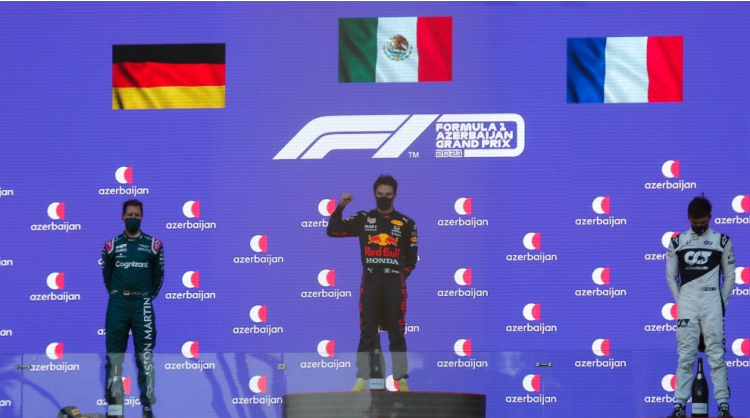
\includegraphics[width=0.75\textwidth]{ideal.png}
    \caption{Proyecto}
    \label{fig:circuito_funcionando}
\end{figure}

\section{Clases implementadas} \label{contenido}
\begin{itemize}
\item \textbf{Imagen:} \\
Atriburos: \begin{itemize}
\item float: ancho, largo, dimenx, dimeny; //Estos atributos son para el manejo de la imagen y para recorrerla
\item vector: rojo, verde, azul; //Vectores para almacenar la intensidad de cada color pixel por pixel
\item vector: rojosin, verdesin, azulesin; //Vectores usados para la verificación de que colores se repiten mas
        \end{itemize}

Métodos:
    \begin{itemize}
        \item analisis(); //Se hace el análisis de la intensidad de colores pixel por pixel y se muestrea en rangos de 16*16.
        \item mostrar(); //Se entregan los datos listos para ser ingresados en tinkercad, se muestra en consola y a su vez se guarda en un archivo .txt
    \end{itemize}

\end{itemize}

\section{Codigo} \label{contenido}
A continuación se mostrarán los códigos implementados para la solución del problema:


\subsection{Qt}
    \begin{lstlisting}[language=C++, label=codigo_ejemplo]
    void Imagen::analisis()
{
    bool band=true;
    float cont1=0,cont2=0;
    int pixelrojo,pixelazul,pixelverde,poselegida,aux0,aux1=0;

    for(int i=0;i<16;i++){ // i filas
        for(int j=0;j<16;j++){// j columnas
            for(cont1=(i*dimenx);cont1<(dimenx*(i+1)-1);cont1++){

                for(cont2=(j*dimeny);cont2<(dimeny*(j+1)-1);cont2++){

                    pixelrojo=imagen->pixelColor(cont1,cont2).red();
                    pixelazul=imagen->pixelColor(cont1,cont2).blue();
                    pixelverde=imagen->pixelColor(cont1,cont2).green();

                    rojo.push_back(pixelrojo);
                    azul.push_back(pixelazul);
                    verde.push_back(pixelverde);
                    if(rojosin.size()==0){
                        rojosin.push_back(pixelrojo);
                        band=false;
                    }

                    else{
                        band=true;
                        for(unsigned int ite=0;ite<(rojosin.size());ite++){
                            if(rojosin[ite]==pixelrojo){
                                band=false;
                            }
                        }
                    }
                    if(band==true) rojosin.push_back(pixelrojo);



                    if(azulsin.size()==0){
                        azulsin.push_back(pixelazul);
                        band=false;
                    }
                    else{
                        band=true;
                        for(unsigned int ite=0;ite<(azulsin.size());ite++){
                            if(azulsin[ite]==pixelazul){
                                band=false;
                            }
                        }
                    }
                    if(band==true) azulsin.push_back(pixelazul);


                    if(verdesin.size()==0){
                        verdesin.push_back(pixelverde);
                        band=false;
                    }

                    else{
                        band=true;
                        for(unsigned int ite=0;ite<(verdesin.size());ite++){
                            if(verdesin[ite]==pixelverde){
                                band=false;
                            }
                        }
                    }
                    if(band==true) verdesin.push_back(pixelverde);

                }
            }
            for(unsigned int it=0;it<(rojosin.size());it++){
                aux0=0;
                for(unsigned int ite=0;ite<rojo.size();ite++){
                    if(rojosin[it]==rojo[ite]){
                        aux0++;
                    }

                }
                if(aux0>aux1){
                    aux1=aux0;
                    poselegida=it;
                }
            }
            Mrojo[i][j]=rojosin[poselegida];
            aux1=0;

            for(unsigned int it=0;it<(azulsin.size());it++){
                aux0=0;
                for(unsigned int ite=0;ite<azul.size();ite++){
                    if(azulsin[it]==azul[ite]){
                        aux0++;
                    }

                }
                if(aux0>aux1){
                    aux1=aux0;
                    poselegida=it;
                }
            }
            Mazul[i][j]=azulsin[poselegida];
            aux1=0;
            for(unsigned int it=0;it<verdesin.size();it++){
                aux0=0;
                for(unsigned int ite=0;ite<verde.size();ite++){
                    if(verdesin[it]==verde[ite]){
                        aux0++;
                    }

                }
                if(aux0>aux1){
                    aux1=aux0;
                    poselegida=it;
                }
            }
            Mverde[i][j]=verdesin[poselegida];
            aux1=0;
            rojo.clear();
            azul.clear();
            verde.clear();
            rojosin.clear();
            azulsin.clear();
            verdesin.clear();
        }

    }

}

void Imagen::mostrar()
{
        string str;
        ofstream archivo;

        archivo.open("bandera.txt",ios::out);

        //////////CODIGO PARA IMPRIMIR 3 ARREGLOS INDIVIDUALES DE 256
        cout<<"byte reds[256] = {";
        archivo<<"byte reds[256] = {";
        for(int i=0;i<16;i++) {
            for(int j=0;j<16;j++) {
                if(i==15 && j==15) {
                    cout<<Mrojo[(j)][(i)]<<"};";
                    archivo<<Mrojo[(j)][(i)]<<"};";
                }
                else {
                    cout<<Mrojo[(j)][(i)]<<",";
                    archivo<<Mrojo[(j)][(i)]<<",";
                }
            }
            cout<<"\n";
            archivo<<"\n";
        }

        cout<<"\n\nbyte greens[256] = {";
        archivo<<"\n\nbyte greens[256] = {";
        for(int i=0;i<16;i++) {
            for(int j=0;j<16;j++) {
                if(i==15 && j==15) {
                    cout<<Mverde[(j)][(i)]<<"};";
                    archivo<<Mverde[(j)][(i)]<<"};";
                }
                else {
                    cout<<Mverde[(j)][(i)]<<",";
                    archivo<<Mverde[(j)][(i)]<<",";
                }
            }
            cout<<"\n";
            archivo<<"\n";
        }

        cout<<"\n\nbyte blues[256] = {";
        archivo<<"\n\nbyte blues[256] = {";
        for(int i=0;i<16;i++) {
            for(int j=0;j<16;j++) {
                if(i==15 && j==15) {
                    cout<<Mazul[(j)][(i)]<<"};";
                    archivo<<Mazul[(j)][(i)]<<"};";
                }

                else {
                    cout<<Mazul[(j)][(i)]<<",";
                    archivo<<Mazul[(j)][(i)]<<",";
                }

            }
            cout<<"\n";
            archivo<<"\n";
        }
}
    
    \end{lstlisting}


\subsection{Tinkercad}
    \begin{lstlisting}[language=C++, label=codigo_ejemplo]
//Incluimos la libreria necesaria para el manejo de las tiras
#include <Adafruit_NeoPixel.h>
//Definimos el pin desde el arduino
int neopixelPin = 2;
//Definimos la cantidad de leds
int no_ofPixels = 256;
//Se hace la inicializacion de los neopixel, con su # de les, y pin
Adafruit_NeoPixel pixels = Adafruit_NeoPixel(no_ofPixels, neopixelPin, NEO_GRB + NEO_KHZ800);


//////////AGREGAR ACÁ LO QUE ENTREGA EL CODIGO DE QT////////////////////

/*En este caso tenemos la de Brasil precargada, se encuentra dividida en 3 arreglos de 256 posiciones correspondientes c/u a un led del arreglo*/
//Bandera Brasil

byte reds[256] = {64,64,64,64,64,64,64,64,64,64,64,64,64,64,64,64,
64,64,64,64,64,64,64,64,64,64,64,64,64,64,64,64,
64,64,64,64,64,64,64,253,253,64,64,64,64,64,64,64,
64,64,64,64,64,64,253,253,253,253,64,64,64,64,64,64,
64,64,64,64,64,253,253,12,12,253,253,64,64,64,64,64,
64,64,64,64,253,253,12,12,12,12,253,253,64,64,64,64,
64,64,64,253,253,253,255,12,12,12,12,253,253,64,64,64,
64,64,253,253,253,12,12,12,255,12,12,253,253,253,64,64,
64,64,253,253,253,12,12,12,12,12,255,253,253,253,64,64,
64,64,64,253,253,12,12,12,12,12,253,253,253,64,64,64,
64,64,64,64,253,253,12,12,12,12,253,253,64,64,64,64,
64,64,64,64,64,253,253,12,12,253,253,64,64,64,64,64,
64,64,64,64,64,64,253,253,253,253,64,64,64,64,64,64,
64,64,64,64,64,64,64,253,253,64,64,64,64,64,64,64,
64,64,64,64,64,64,64,64,64,64,64,64,64,64,64,64,
64,64,64,64,64,64,64,64,64,64,64,64,64,64,64,64};


byte greens[256] = 
{140,140,140,140,140,140,140,140,140,140,140,140,140,140,140,140,
140,140,140,140,140,140,140,140,140,140,140,140,140,140,140,140,
140,140,140,140,140,140,140,223,223,140,140,140,140,140,140,140,
140,140,140,140,140,140,223,223,223,223,140,140,140,140,140,140,
140,140,140,140,140,223,223,82,82,223,223,140,140,140,140,140,
140,140,140,140,223,223,82,82,82,82,223,223,140,140,140,140,
140,140,140,223,223,223,255,82,82,82,82,223,223,140,140,140,
140,140,223,223,223,82,82,82,255,82,82,223,223,223,140,140,
140,140,223,223,223,82,82,82,82,82,255,223,223,223,140,140,
140,140,140,223,223,223,82,82,82,82,223,223,223,140,140,140,
140,140,140,140,223,223,82,82,82,82,223,223,140,140,140,140,
140,140,140,140,140,223,223,82,82,223,223,140,140,140,140,140,
140,140,140,140,140,140,223,223,223,223,140,140,140,140,140,140,
140,140,140,140,140,140,140,223,223,140,140,140,140,140,140,140,
140,140,140,140,140,140,140,140,140,140,140,140,140,140,140,140,
140,140,140,140,140,140,140,140,140,140,140,140,140,140,140,140};


byte blues[256] = {65,65,65,65,65,65,65,65,65,65,65,65,65,65,65,65,
65,65,65,65,65,65,65,65,65,65,65,65,65,65,65,65,
65,65,65,65,65,65,65,1,1,65,65,65,65,65,65,65,
65,65,65,65,65,65,1,1,1,1,65,65,65,65,65,65,
65,65,65,65,65,1,1,131,131,1,1,65,65,65,65,65,
65,65,65,65,1,1,131,131,131,131,1,1,65,65,65,65,
65,65,65,1,1,1,255,131,131,131,131,1,1,65,65,65,
65,65,1,1,1,131,131,131,255,131,131,1,1,1,65,65,
65,65,1,1,1,131,131,131,131,131,255,1,1,1,65,65,
65,65,65,1,1,1,131,131,131,131,1,1,1,65,65,65,
65,65,65,65,1,1,131,131,131,131,1,1,65,65,65,65,
65,65,65,65,65,1,1,131,131,1,1,65,65,65,65,65,
65,65,65,65,65,65,1,1,1,1,65,65,65,65,65,65,
65,65,65,65,65,65,65,1,1,65,65,65,65,65,65,65,
65,65,65,65,65,65,65,65,65,65,65,65,65,65,65,65,
65,65,65,65,65,65,65,65,65,65,65,65,65,65,65,65};
////////////////////////////////////////////////////////////

void setup() {
  //inicializamos
  pixels.begin();
  
  for (int i=0;i<no_ofPixels;i++){
  //si los valores de RGB son iguales debemos tener eso en cuenta
    if(reds[i]==greens[i] && reds[i]==blues[i]){
      if(reds[i]>0) //si son mayores a 0, le restamos 1 al rojo
        pixels.setPixelColor(i, reds[i]-1, greens[i],blues[i]);
      else //si son 0, le sumamos 1 al rojo
        pixels.setPixelColor(i, reds[i]+1, greens[i],blues[i]);
    }
  else //en caso de que no se cumpla ninguna de 
  //las condiciones hacemos la muestra de forma normal
    pixels.setPixelColor(i, reds[i], greens[i],blues[i]);
  }
  //encendemos todos los leds despues hacer la carga de los valores
  pixels.show();  
}
\end{lstlisting}

\section{Estrucutura circuito}\label{images}
    El circuito se compone de :
    \begin{itemize}
    \item Arduino Uno R3
    \item Tira de 16 NeoPixel *12
    \end{itemize}
    \begin{figure}[h]
    \centering
    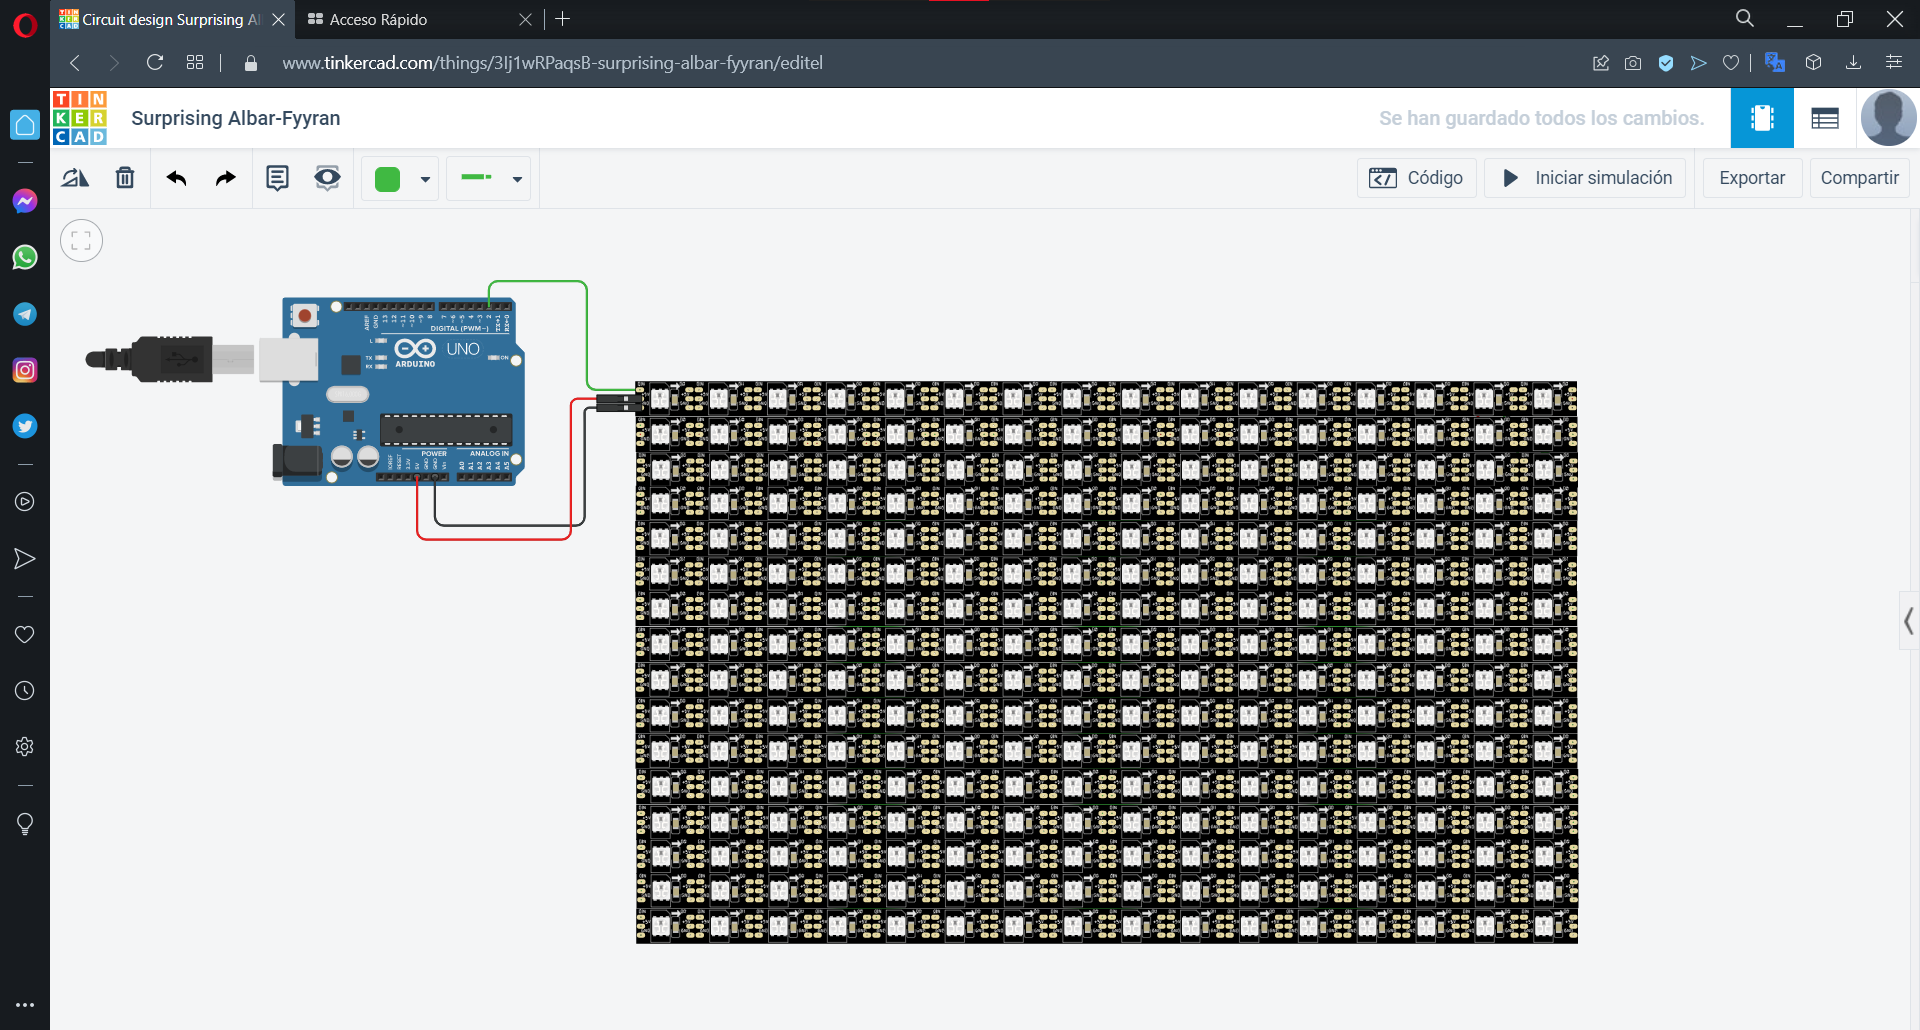
\includegraphics[width=1.2\textwidth]{montaje.png}
    \caption{Montaje circuito}
    \label{fig:montaje}
    \end{figure}
    
    \begin{figure}[h]
    \centering
    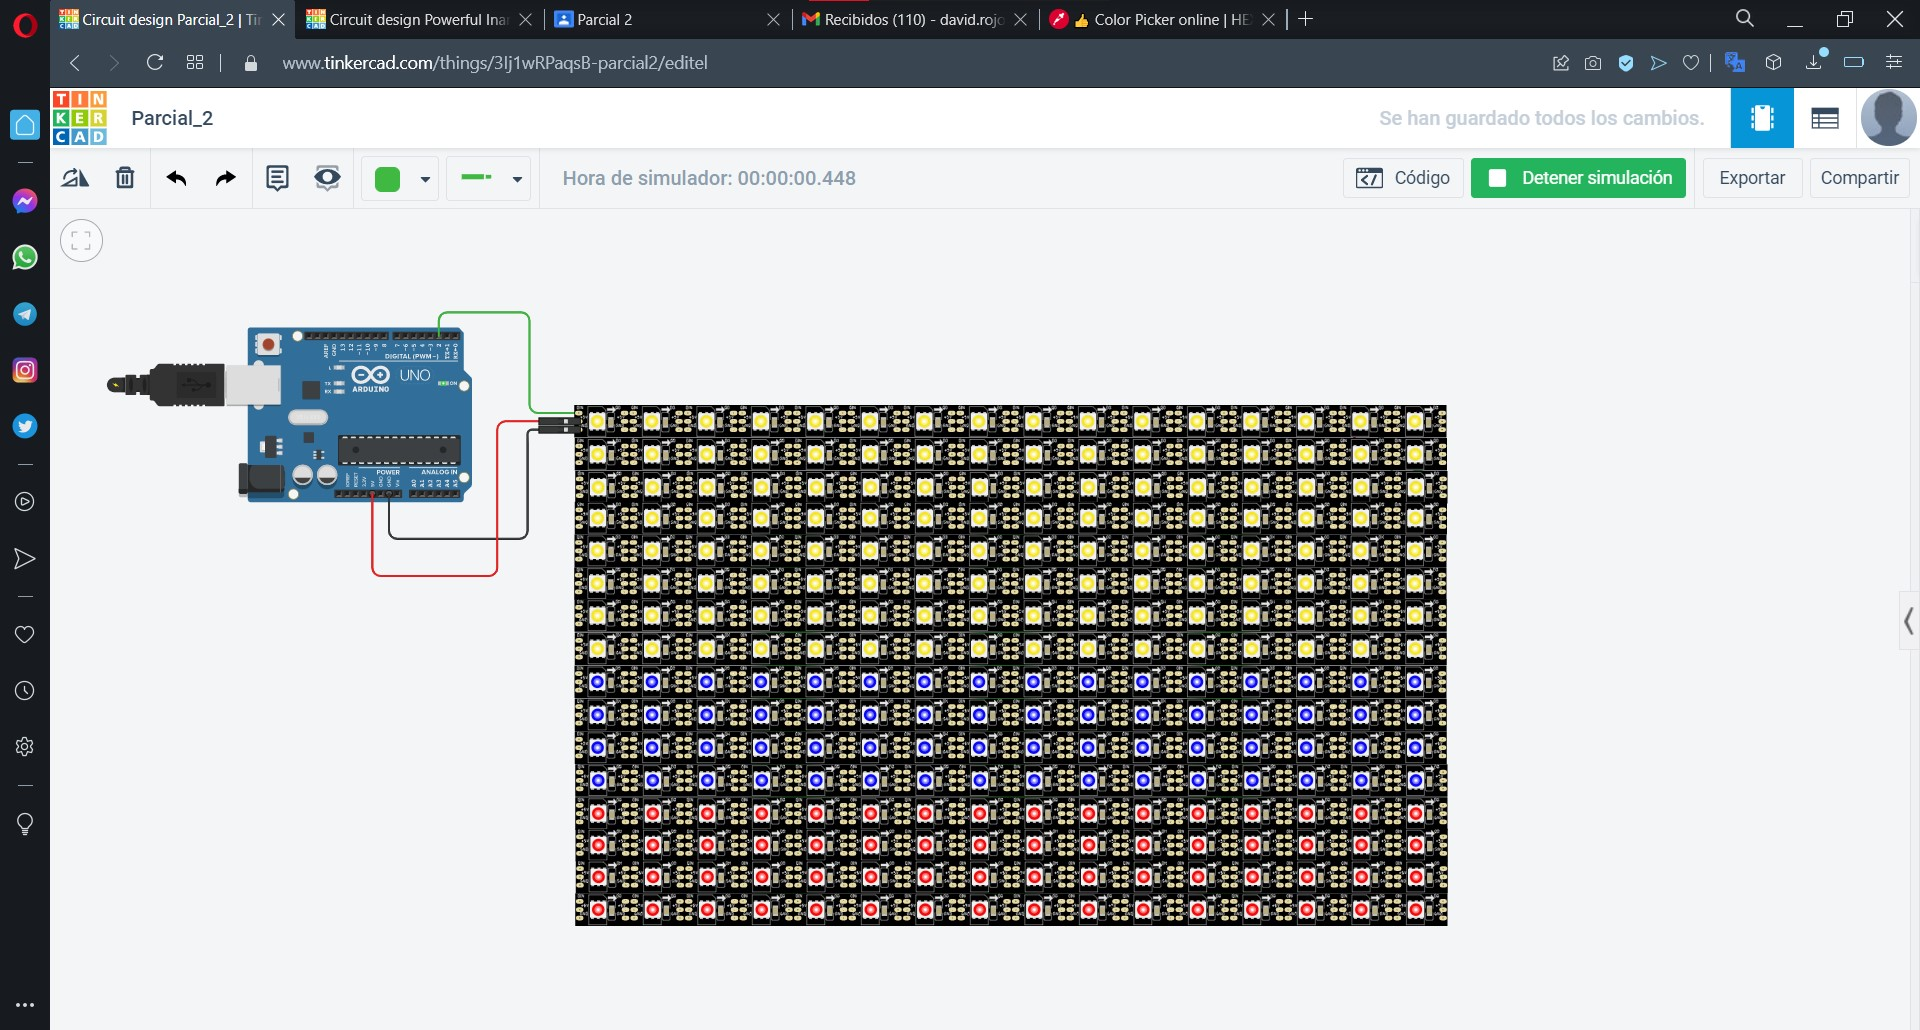
\includegraphics[width=1.2\textwidth]{circuito en funcionamiento.jpg}
    \caption{Circuito en funcionamiento}
    \label{fig:circuito_funcionando}
    \end{figure}


\section{Problemas presentados}
\begin{itemize}
    \item Principalmente se evaluó si era necesario la inserción de una fuente para una correcta alimentación del circuito, pero se descarta, ya que para la cantidad de tiras empleadas el arduino tiene la capacidad de alimentarlas sin problema.
    \item Se presentaron problemas al intentar almacenar el total de los valores en un solo arreglo [256][3], como si se estuviera accediendo a un máximo de memoria limitada, por lo tanto se lleva a cabo la solución en 3 arreglos individuales de [256], con este cambio se logró un funcionamiento correcto.
    \item En algunos casos se aprecia que al repetirse constantemente el mismo número en los 3 colores se puede llegar a presentar una inconsistencia, por lo tanto se agregan condicionales para evitar este posible inconveniente
    \item Se presenta problema a la hora de proyectar banderas que contengan el color negro, ya que este se representa a través de la ausencia de todos los colores (R=0; G=0; B=0), pero en la simulación a través de Tinkercad con esta ausencia total de color, representa el bombillo apagado, que a simple vista se aprecia como color blanco \textit{(como se muestra en la figura 4)}
    \item Otros errores que se presentaron fue en la implementación del código en Qt, pequeños errores de ciclos infinitos, o de crasheo por manejo erróneo de contenedores.
    \begin{figure}[h]
    \centering
    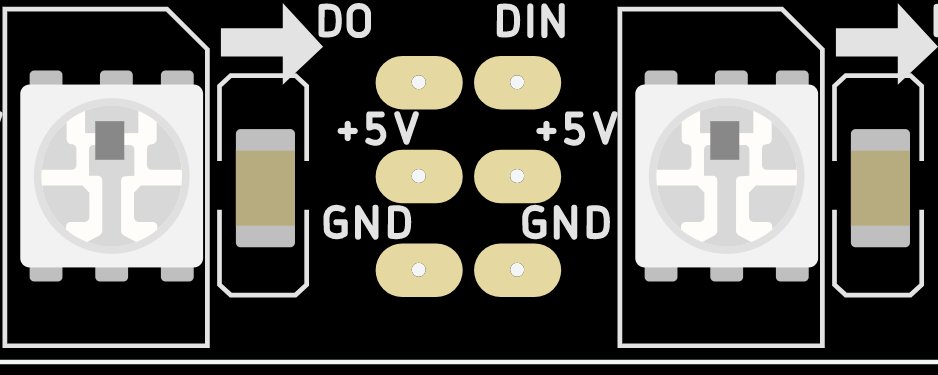
\includegraphics[width=0.5\textwidth]{error1.png}
    \caption{Izquierda:RGB(0,0,0) --- Derecha:Led Apagado }
    \label{fig:error1}
    \end{figure}
    \item Más que un problema, uno de los puntos más importantes a tener en cuenta en el diseño del montaje es la inclusión de una fuente, en este caso se hizo una análisis para saber si era lo indicado o no para nuestra situación \textit{como se puede ver en la figura 5}, A la izquierda tenemos nuestro arreglo de 16*16 con la representación de la bandera de Colombia, a la derecha tenemos un pequeño arreglo de tan solo dos tiras Neopixel en las cuales se está representando el color rojo con las mismas intensidades \textit{(que a la izq)}, en ambos casos el color rojo que se aprecia tiene exactamente la misma intensidad, lo que muestra que el hecho de tener 256 LEDs alimentados no hace que pierda intensidad el color.
     \begin{figure}[h]
    \centering
    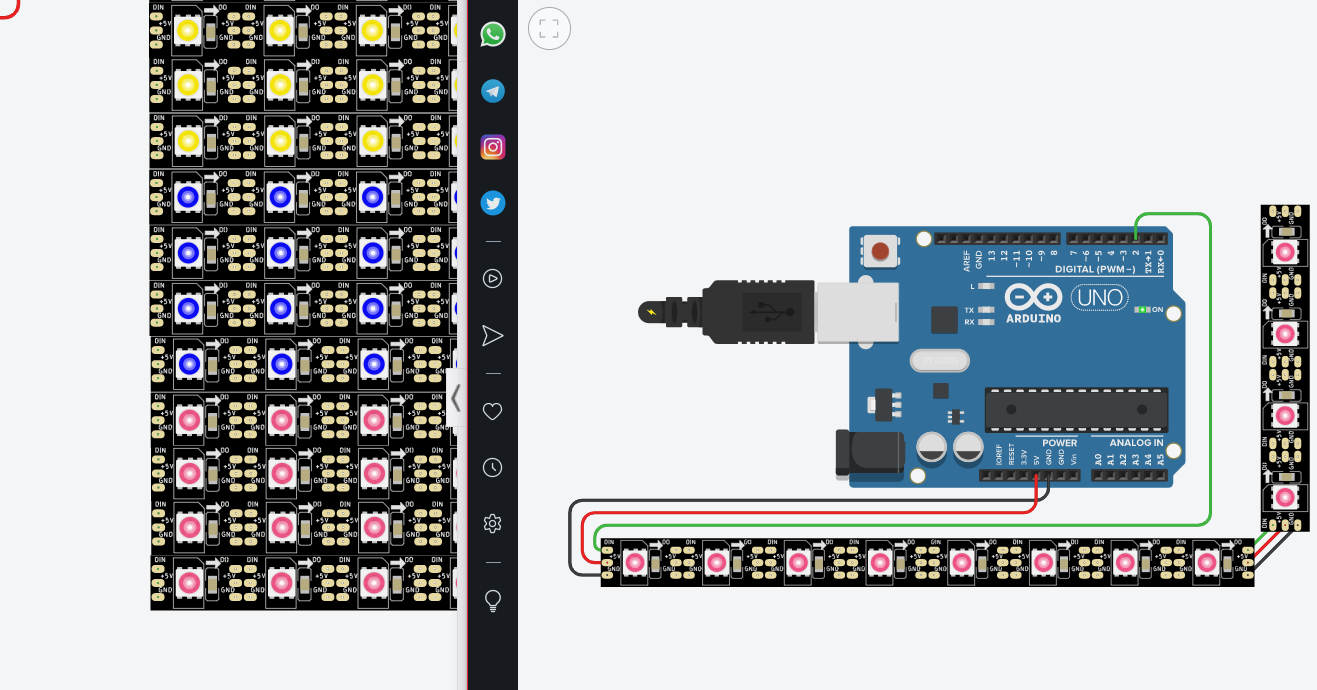
\includegraphics[width=1\textwidth]{analisis.png}
    \caption{Análisis incersión fuente }
    \label{fig:error1}
    \end{figure}
    \item Debido al problema del color negro ya antes mencionado, surgía la posibilidad de corregirlo, generando condicionales para que cuando los valores sean R=0, G=0, B=0, se cambiará por una tonalidad gris, lo más similar posible al negro, pero este condicional solo funcionaria en algunos casos específicos, ya que el color negro de la bandera no siempre viene representado por (0,0,0) por ende preferimos no agregar el condicional y tener en cuenta que en caso de querer presentar imágenes con detalles negros se deberá hacer una configuración más especifica, pero ya conociendo los casos que hay que tener en cuenta.
\end{itemize}

\end{document}
